\documentclass[12pt,a4paper,twoside]{report}
\usepackage[utf8]{inputenc}
\usepackage[portuguese]{babel}
\usepackage[T1]{fontenc}
\usepackage{fancyhdr}
\usepackage{amsmath}
\usepackage{amsfonts}
\usepackage{amssymb}
\usepackage{makeidx}
\usepackage{graphicx}
\usepackage{lmodern}
\usepackage{wrapfig}
\usepackage{color}
\usepackage{float}
%\usepackage{fourier}
\usepackage[left=2cm,right=2cm,top=2cm,bottom=2cm]{geometry}
\author{Bartolomeu J. Ubisse}
\pagestyle{fancy}
\renewcommand{\headrulewidth}{0pt}
\renewcommand{\footrulewidth}{1pt}
\fancyfoot[L]{ | UEM - 2017}
\fancyfoot[c]{}
\fancyfoot[r]{\thepage}
\begin{document}


\begin{figure}[htb]

\centering

\includegraphics[scale=1]{UEM-logotipo}
\end{figure}
\centering
{ \Large Universidade Eduardo Mondlane}\\[0.3cm] 
\large Faculdade de Ci\^encias\\[0.2cm]
 \large Departamento de F\'isica\\[0.5cm]

%\textsc{Electr\^onica B\'asica} \\[1cm]
\begin{flushleft}
\tt Teste 1 - E. Anal\'ogica\hspace{0.25cm} |Data:$05/04/2017$\hspace{0.25cm}|Hora:$10:00-12:00$ hrs.\\
\hrulefill
\end{flushleft}

\begin{enumerate}
\item Dado o circuito da fig.\ref{f2}, determine: $i)$ O equivalente Thevenin e a queda de tensão na resistência de carga; $ii)$ A queda de tensão na resistência de carga usando o princípio de superposição.[$4.0$ Valores]
\begin{figure}[H]
\centering
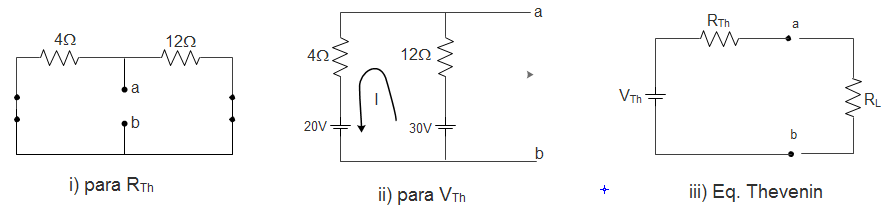
\includegraphics[scale=1]{Thevenin}
\caption{}
\label{f2}
\end{figure}
\item Explique o que entende por energia da banda proibida e fa\c ca uma compara\c c\~ao da mesma para os diferentes materiais (ex: $E_{g-A}>E_{g-B}>E_{g-C}$, onde $A$,$B$ e $C$ s\~ao os materiais).[$2.0$ Valores]
\item A forma encontrada at\'e ent\~ao de se melhorar de uma maneira controlada a condutibilidade de um material semicondutor \'e a dopagem. Explique como \'e poss\'ivel obter um material de sil\'icio de tipo $P$ e indique os portadores maiorit\'arios e o tipo de i\~oes presentes no mesmo.[$2.0$ Valores]
\item Explique o processo de surgimento de barreira de potencial numa jun\c c\~ao $PN$.[$2.0$ Valores]
\item Imagine que um dia o seu pai, por saber que voc\^e frequenta a cadeira de electr\^onica, solicite que verifique se o d\'iodo do seu r\'adio est\'a ou n\~ao danificado. Isto porque um t\'ecnico amador da sua rua o ter\'a dito que o problema era desse d\'iodo. Explique de que forma voc\^e pode fazer esse diagn\'ostico considerando que na sua casa tem um m\'ultimetro digital.[$3.0$ Valores]
\item Considere um circu\'ito retificador de onda completa cujo  sinal de entrada \'e de $60 Hz$ e o de saida tem um valor de pico de $10V$. Determine a capacit\^ancia do capacitor do filtro de modo que o ripple do sinal de sa\'ida seja: i) $V_r=0.2V$ e ii) $V_r=0.5V$. Se todos esses capacitores estivessem ao seu dispor, qual deles usaria para o seu circu\'ito retificador? Porqu\^e? Considere a carga de $2k\Omega$.[$3.0$ Valores]
\item Para o circuito da fig.\ref{f1}, determine as tensões de entrada (a mínima e a máxima) de modo que o díodo Zener funcione correctamente regulando a tens\~ao.[$3.0$ Valores]
\begin{figure}[H]
\centering
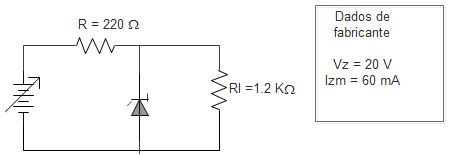
\includegraphics[scale=1]{cZener}
\caption{Circu\'ito regulador}
\label{f1}
\end{figure}

\begin{enumerate}
\item[a)]Esboce a forma do sinal de entrada no regulador da fig.\ref{f1} em fun\c c\~ao do tempo e indique o ripple correspondente.[$1.0$ Valores]
\end{enumerate}


\end{enumerate}

\vspace{4cm}

\Huge{Bom Trabalho !}




\end{document}